\documentclass[12pt]{article} 
\usepackage{amsfonts, amsmath, amssymb} 
\usepackage{dcolumn, multirow} 
\usepackage{setspace} 
\usepackage{epsfig, subfigure, subfloat, graphicx}
\usepackage{tabularx} 
\usepackage{anysize, indentfirst, setspace} 
\usepackage{verbatim, rotating, paralist}
\usepackage{latexsym} 
\usepackage{amsthm} 
\usepackage{fullpage} 
\usepackage{longtable} 
\usepackage{graphicx} 
\usepackage{mathabx} 
\usepackage{txfonts} 
\usepackage{amsfonts} 
\usepackage{parskip} 
\usepackage{stmaryrd} 
\usepackage{mathrsfs} 
\usepackage{dsfont} 
\usepackage{comment} 
\usepackage{url} 
\usepackage{rotating} 
\usepackage{appendix}
\usepackage{natbib} 
\usepackage{tablefootnote}
\usepackage{hyperref}



\usepackage[margin=2.5cm]{geometry}

\title{ArcPy Introductory Tutorial}
\author{Nick Eubank}
\date{\today}


\begin{document} 
\maketitle

\tableofcontents

\section{Introduction: What is ArcPy?}

\begin{center}
\emph{Note to readers: if you already know what ArcPy is about, are confident you have ArcPy installed, and just want to get started, feel free to skip ahead to Section 2}
\end{center}


ArcPy is a tool for telling ArcGIS what to do using Python instead of interacting with ArcGIS by clicking on toolboxes in the graphical user interface (GUI). In other words, it's a way to write code for ArcGIS in the same way that you write code for Stata or R. 

There are lots of different ways to use ArcPy, from the very simple to the very complex. I think the most important thing for people to understand is that no matter your level of programming and computer science sophistication, there's a way ArcPy can be of use to you. 

With that in mind, this tutorial starts with how to use ArcPy for it's most basic purpose -- writing ArcPy \emph{scripts}. Scripts are the most basic type of program you can imagine -- a series of commands that are executed in a linear, deterministic fashion. That means no ``if'' clauses, no ``while'' loops, and nothing else complicated -- just a list of the things you would otherwise be doing with a mouse.\footnote{If you like analogies, you can think of most programs as being like \emph{Choose Your Own Adventure} books, where depending on input from the user, or what's in the data, the story may evolve in different ways. A script is just a regular novel -- the same every time.} In addition to starting with simple programs, we'll also walk through how to get ArcGIS to actually write your ArcPy scripts for you.  Then after you've developed a complete, self-sufficient toolset for working with ArcPy in this simple way, we will explore different extensions. 

One important clarification about ArcPy I've found people find helpful: ArcPy is not a Python-based alternative to ArcGIS; it's just a tool for using Python to \emph{tell ArcGIS what to do}. Think of ArcPy as a friend sitting at your computer, clicking on those toolboxes in ArcGIS on your behalf. That's why ArcPy doesn't work without ArcGIS installed on the same system. 

\subsection*{Why Use ArcPy?}
In my view, there are three reasons to use ArcPy instead of clicking on boxes with your mouse (i.e. using the GUI):
\begin{enumerate}
	\item \textbf{Save Time} \\
	We have all been in the situation where, after several days of work in ArcGIS, we suddenly realize we need to make a small change to one of the first steps in a project. If you're using the GUI, you have to go through and re-do \emph{everything}. But if you're working in ArcPy, you can modify that initial step in your code, hit run, and everything gets updated. You may not want to use ArcPy when you're doing data exploration, but any time you're setting up something with more than a couple steps, I would highly recommend doing it in ArcPy. 
	\item \textbf{Protect Yourself from Mistakes} \\
	I have found many social scientists' strategy for avoiding mistakes is to ``just be careful.'' But to err is human, and I think it is better to \emph{assume} you'll make mistakes, and to design systems to help you catch them. \\
	In the ArcGIS GUI, all mistakes are ephemeral -- if you don't catch them the moment they are made, all record of them is gone. But if you code in ArcPy, then you have a record of what you've done you can go back and check later. You wouldn't write a paper without proofreading it the next day -- why could you program that way?
	\item \textbf{Replicability} \\
	Creating fully replicable results is where social science is headed, and ArcPy is the only way you can write replication code for ArcGIS. It's not required by most journals yet, but it's only a matter of time. 
\end{enumerate}


\subsection*{Before You Start}
This tutorial assumes that you've already:
\begin{itemize}
	\item Installed ArcGIS version 9.x or 10.x (i.e. some iteration of ArcGIS version 9 or version 10)
	\item Installed a Python ``Interactive Development Editor'' (IDE) like PyScripter, PyCharm, or Canopy where you can edit, run, and debug your ArcPy files. 
	\begin{itemize}
		\item Note you don't (indeed shouldn't) install Python itself -- ArcGIS already did that, and if you try to re-install Python, it will just confuse things. 
		\item If you're working on a Mac and running ArcGIS in Parallels Desktop, Bootcamp or similar software, you need to install the IDE in Windows. Sadly, ArcPy does not (yet) reach across the operating system barrier. 
	\end{itemize} 
	\item Have a \emph{basic} understanding of Python. You \emph{really} don't need to know much, but a little exposure necessary. 
\end{itemize}

You can test for whether ArcPy is installed by just running the following command in your Python IDE: 
\begin{verbatim}
	import arcpy
\end{verbatim}

If it works, you're good, and you can move on. If not, go to the ArcPy\_InstallationTroubleshooting.pdf document. 

\pagebreak
\section{Scripting in ArcPy by Copy-Paste}\label{scripting}

ArcGIS has a great tool for introducing people to ArcPy -- it writes your code for you! To illustrate, let's make an ArcPy script to create a Personal Geo-Database. 

\subsubsection*{Set Up Your ArcPy Script} 
First, make a new Python file in your IDE, and add the following two lines to the top (the carrots ($>$) are included to denote separate lines -- do not include them in your code!):
\begin{quote}
\begin{verbatim}
> import arcpy
> arcpy.env.overwriteOutput = True
\end{verbatim}	
\end{quote}
These two commands will (a) import the arcpy toolset, and (b) set ArcPy to overwrite old files if you try to create something that's already there.\footnote{Stata users can think of it as a global ``, replace''.} 

\subsubsection*{Do What You Want to Do In ArcMap}
This you (hopefully) know how to do -- just open ArcMap, open the toolboxes, select the ``Workspace'' toolbox folder, and select ``Create Personal GDB.'' Call your database something creative (I'll call mine ``myDatabase'') and save it. 

Note you \emph{do} need to create the database by clicking on the ``Create Personal GDB'' toolbox -- ArcGIS only creates snippets for things created by clicking on toolboxes. If you were to just right-click on a folder and select \emph{New $>$ Personal Geodatabase} in the catalogue window, no code will be generated. 

\subsubsection*{Retrieve the Python Snippet}
OK, now the new part: when you executed that tool, ArcGIS actually saved a copy of the ArcPy command for that action -- we just need to get it. 
\begin{enumerate}
	\item Open the ``Results'' display by going to the Geoprocessing Menu and selecting ``Results.'' \\
	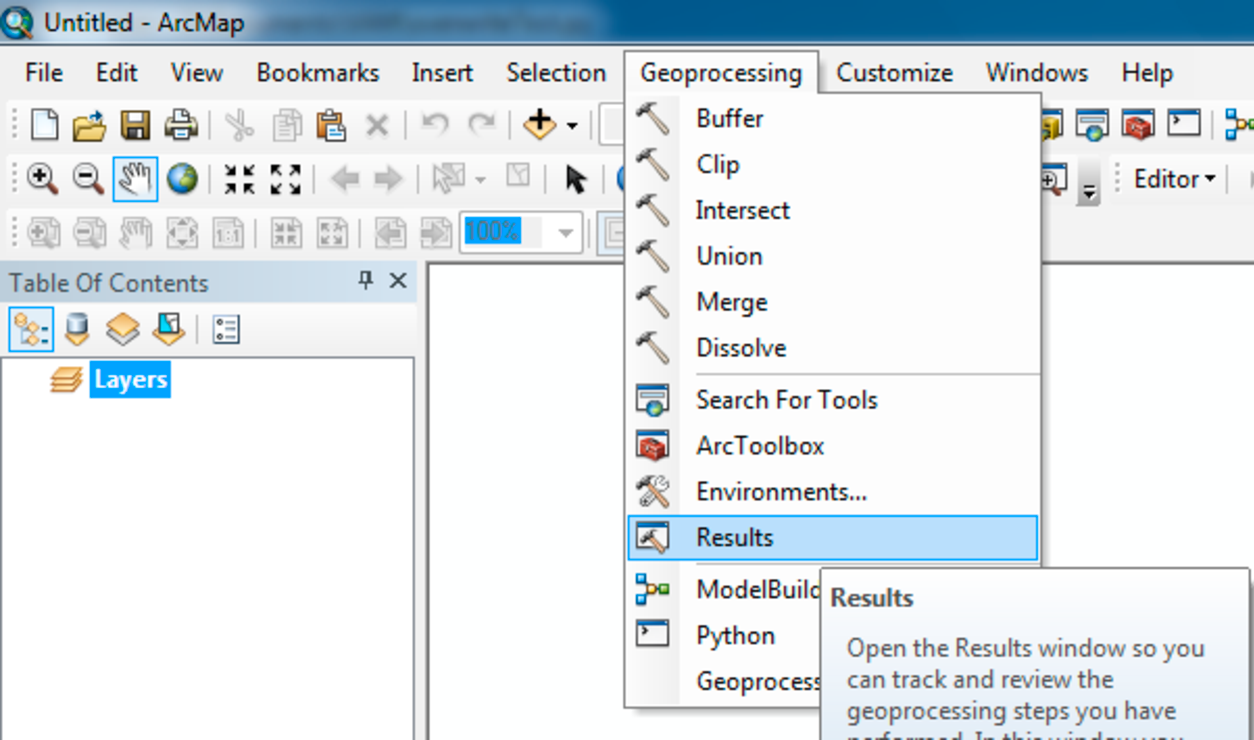
\includegraphics[scale=.4]{figures/resultsMenu.pdf}  
	\item Click the check box next to ``Current Session'' so you can see the command you just executed. \\
	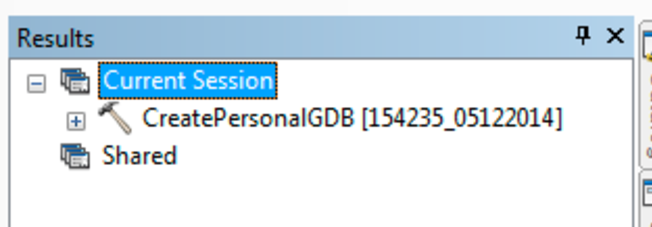
\includegraphics[scale=0.8]{figures/results2.pdf} \\
	\item Right click on the command you just executed and select ``Copy As Python Snippet.'' \\
	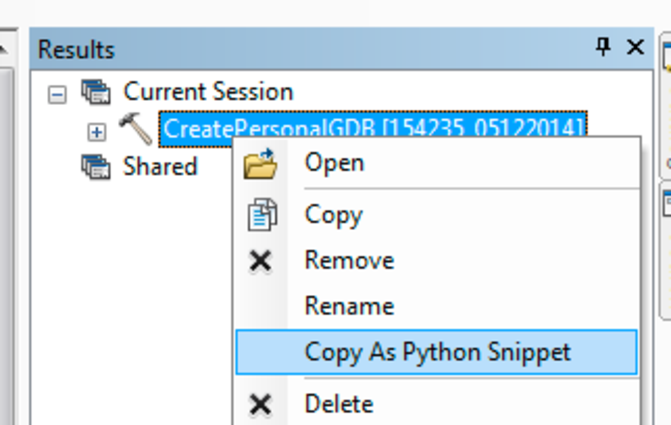
\includegraphics[scale=0.8]{figures/results3.pdf} \\
	\item Now just go back to your Python file and paste the result! \\
	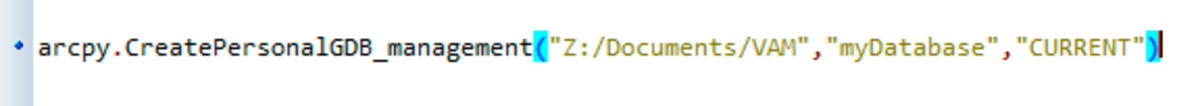
\includegraphics[scale=0.8]{figures/paste1.pdf}
\end{enumerate}
Congratulations! You now have a viable ArcPy script! And really, that's all there is to it. As long as you execute a command in ArcMap by opening a toolbox, you should be able to copy the associated Python snippet from the results menu. 

\subsubsection*{Running Your ArcPy Script}
There's a small trick to running ArcPy scripts -- before you run them, you \emph{probably} need to close all open ESRI products. 

Whenever a file is being used by an ESRI product, Arc will place a ``schema lock'' on that file. This stops anyone else from trying to modify that file while someone else has it open (to prevent simultaneous edits from corrupting a file). That means that if ArcMap is open and has a schema lock on a file, anything you do in ArcPy with that file will fail (and no, it often won't tell you that it's because of a schema lock).

Moreover, ArcGIS is very aggressive in placing schema locks on things, so even if you don't think a file is open in ArcMap and so there shouldn't be a lock on it, so long as ArcMap is open, there's a good chance there's a lock on your files.\footnote{For example, anything you opened and then closed in ArcMap usually keeps its lock till you actually close ArcMap, and sometimes if ArcMap had to just reference a file to populate it's Catalogue tree, it will put a lock on it.} So it's just good practice to always close everything before you run your scripts. 
 
\pagebreak
\section{Scripting Directly in ArcPy}
The Copy-Paste trick is the safety-net of ArcPy -- something that's great to have available, but not the place you want to spend all your time. The reason is that it has a number of limitations: it's cumbersome if you want to write ArcPy scripts directly, and copy-pasted code can be hard to read, interpret, and modify. 

\subsection*{Learning and Deciphering Commands}
Your best friend when working in ArcPy is the \href{http://help.arcgis.com/en/arcgisdesktop/10.0/help/index.html}{\underline{ESRI help site}}. I recommend just leaving a browser open at all time when working in ArcPy.\footnote{To navigate the ESRI site, I actually recommend googling ``arcgis [name of tool you're interested in]'', and follow the ``Desktop Help'' link that is usually near the top of the results.}

On the page for a tool you will find a \emph{Syntax} section that will describe the syntax for each tool's ArcPy command. For example, if I were to go to the site for the ``Create Personal GeoDatabase'' tool, I would see the following in the middle of the page: 

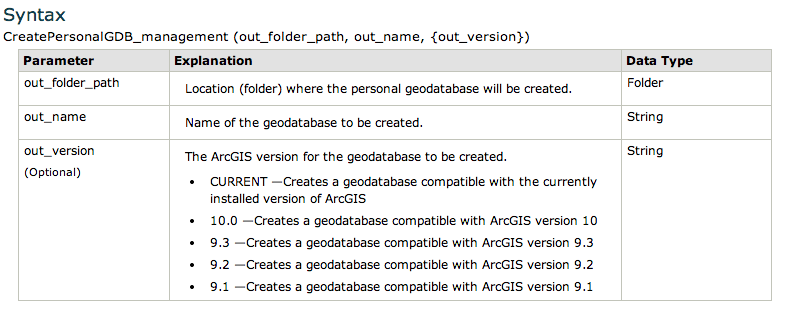
\includegraphics[scale=0.5]{figures/helpSyntax.png}

The first line below Syntax tells me: 
\begin{itemize}
	\item The command for creating a Personal Database is ``CreatePersonalGDB\_management()'', which means I would call it as ``arcpy.CreatePersonalGDB\_management()'' in my ArcPy script. 
	\item The first argument is the filepath of the folder in which I want the geodatabase located
	\item The second argument is the name of the geodatabase
	\item And the third argument (which is optional, as indicated by squiggly brackets) is the version. 
\end{itemize}

The table below provides detailed information on each of the arguments of the function. So from the third row, we can see that \emph{out\_version} is the version of ArcGIS with which we want the database to be compatible, the function is looking for the value in that position to be a string, and the acceptable values of that string are ``CURRENT'', ``10.0'', ``9.3'', ``9.2'', and ``9.1''.

Finally, each help site also includes one or two examples of the function being used in a Python script below these boxes, which can also be extremely helpful. 

\section{Good Hygiene}\label{hygiene}
A critical practice in ArcGIS is to start all projects by copying your source data from a safe place to a working folder where you can make modifications without worrying about corrupting your source data. This is far more important in ArcGIS than in software like R or Stata because (unlike those applications) ArcGIS has lots of tools that will modify their source files \emph{without asking!} So you should \emph{never} work directly with your source data. 

(Note this isn't actually specific to ArcPy, but it's worth reiterating!)

\section{Style}
Good ``style'' helps keep code readable and helps us avoid mistakes. Unfortunately, code we copy-paste from ArcMap is not code with style we want to emulate. For example, consider the following Python snippet generated when I attempted to define the coordinate system for a feature class called ``myExampleFeature'' to WGS 1984. The command only has two arguments -- the target feature class and the coordinate system to assign -- but it comes out almost unreadable:

\begin{quote}
\begin{verbatim}
> arcpy.DefineProjection_management("Z:/Documents/VAM/test2.gdb/myExample
Feature","GEOGCS['GCS_WGS_1984',DATUM['D_WGS_1984',SPHEROID['WGS_1984',
6378137.0,298.257223563]],PRIMEM['Greenwich',0.0],UNIT['Degree',0.01745
32925199433]]")
\end{verbatim} 
\end{quote}

That's incredibly hard to read, which means it's a good place for mistakes to hide. Fortunately we can clean it up a lot with two small tricks.

\subsection*{\textbf{Set a Working Directory}} 
A working directory is the folder ArcPy will look to first if you give it an incomplete filepath (i.e. a filepath that doesn't start with the drive letter, C or Z). If most of your files are in a certain folder, setting a working directory once helps save you the trouble of writing out full filepaths every time you refer to a file. This is just like $cd$ in Stata or $setwd()$ in R. 

You set the working directory by setting the value of the $arcpy.env.workspace$ variable, as in the following example where I set the working directory to the VAM folder on the Z drive, then drop the prefix from the filepath in the DefineProjection command:   
	\begin{quote}
	\begin{verbatim}
	> arcpy.env.workspace = "Z:/Documents/VAM/"	

	> arcpy.DefineProjection_management("myDatabase.gdb/myExampleFeature",
	"GEOGCS['GCS_WGS_1984',DATUM['D_WGS_1984',SPHEROID['WGS_1984',
	6378137.0,298.257223563]],PRIMEM['Greenwich',0.0],UNIT['Degree',0.01745
	32925199433]]")
	\end{verbatim}
	\end{quote}
OK, that's almost readable!

\subsection*{\textbf{Use a Projection / Coordinate System Variable}}
ArcPy has a tool for storing projections and coordinate systems as single variables called ``Spatial Reference''. The argument takes as input the string name of a coordinate system or projection, and as output creates a coordinate variable.  Since coordinate systems are the ugliest thing to come out of ArcMap snippets, I really love this trick.\footnote{In my experience, just using the name of the spatial reference system you see in ArcMap menus works fine, but you can also find a list of Projected Coordinate System names (and codes -- you can use the second column instead of the name if you want) here: \url{http://resources.arcgis.com/en/help/main/10.1/018z/pdf/projected_coordinate_systems.pdf} ; and Geographic Coordinate Systems here: \url{http://resources.arcgis.com/en/help/main/10.1/018z/pdf/geographic_coordinate_systems.pdf} }	

\begin{quote}
\begin{verbatim}
> arcpy.env.workspace = "Z:/Documents/VAM/myDatabase.gdb"	
> WGS84 = arcpy.SpatialReference('WGS 1984')
> arcpy.DefineProjection_management("myExampleFeature",WGS84)
\end{verbatim}
\end{quote}
There, code we can read. (Two more less important style suggestions can also be found in Section~\ref{morestyle}). 


\section{Editing Fields}
Finally, we often want to calculate, add, or delete fields in our feature attribute tables. Personally, I prefer to avoid doing this in ArcGIS as much as possible -- I prefer to export my data and do field manipulations in Stata -- but if sometimes you just need to do things in ArcGIS. There are three main commands, syntax for which can be found on the ESRI site:
\begin{itemize}
	\item Add a field (prior to calculating): AddField\_management()
	\item Calculate Field: CalculateField\_management()
	\item Delete Field: DeleteField\_management()
\end{itemize}

\section{Cartography}\label{cartography}
Finally, you may not have noticed, but up until now we've mostly been manipulating our data, not its graphical representation. In other words, we haven't really been doing ``cartography,'' the manipulation and creation of actual graphic maps. Fortunately, ArcPy can handle cartography too using the \emph{mapping} library, functions from which you can identify because they require the prefix ``arcpy.mapping.[functionName]'' rather than our usual ``arcpy.[functionName].'' 

When doing cartography, the target of our manipulations is a Map Document, which has the suffix .mxd. You can create a \emph{map} variable (object) that refers to a map document (in this case one I had already created and saved in ArcMap) using the following code: 
\begin{verbatim}
> mxd = arcpy.mapping.MapDocument("Z:/VAM/myMapDocument.mxd")
\end{verbatim}

I'm not going to spend much time on this topic since, honestly, I have only a very limited understanding, but if you do lots of map-making, it's important to know these tools exist! 

Note you can go back and forth from the GUI to ArcPy. So if you want you can setup a map to be very aesthetically appealing by hand, then move into ArcPy to programmatically export PDF maps of each little town on the larger map.  Indeed, if you want an example of map manipulation, the last section of the ``Useful ArcPy Commands and Code Snippets'' PDF is an example of code I wrote to do exactly that -- cycle through constituencies in a map, zoom to their extent, and print a PDF of that particular constituency. 

With that said, here are some example tools:
\begin{itemize}
	\item Create Map Document Variable: mapping.MapDocument(``file.mxd'') \\
	\emph{e.g. mxd = arcpy.mapping.MapDocument(``file.mxd'')}
	\item Set the extent of the Map Document (i.e. zoom) to extent of selected elements of a layer (called myLayer): 
	\begin{quote}
	\begin{verbatim}
		lyrExtent=myLayer.getSelectedExtent()
		df.extent=lyrExtent
	\end{verbatim}		
	\end{quote}
\end{itemize} 

\section{Other Libraries / Modules}
Some tools (like the \emph{mapping} library just discussed) live in special libraries / modules. When calling a tool from one of these other libraries, note you'll need to add an extra prefix (like ``arcpy.mapping.[functionName]'' for \emph{mapping} functions or ``arcpy.sa.[functionName]'' for Spatial Analyst tools). A few you may see include the \emph{mapping} module, the \emph{Spatial Analyst} module (``arcpy.sa.[functionName]''), and the Geostatistical Analyst module (``arcpy.ga.[functionName]''). 

Aside from the need to add prefixes to some commands, you don't need to worry about these different libraries / modules too much -- they're basically just the folders ESRI used to organize its functions when it was writing ArcPy. 

\section{Layers}

One of the least intuitive data structures in ArcGIS is the Layer, and in my experience many people used to working with the ArcGIS GUI don't have a very clear sense of what layers are, which tends to cause problems in ArcPy. With that in mind, this section provides a quick refresher on layers, then discusses the use of layers in ArcPy specifically. 

\subsection*{Background: A Refresher on Layers}

Two things make layers odd. The first is that each layer actually has two components -- the name of a data file (a shapefile, raster, table, etc.) with which is associated, and some additional information about how ArcGIS should work with that file.\footnote{For the Computer Science trained people: layers include a reference/pointer to a source file, and then additional meta-data for that file.} In many (but not all) cases, this additional information pertains to how a data file should be displayed -- what colors and symbols to use, etc. 

The second odd thing about layers is that they are often temporary, and they don’t usually live on the hard drive as independent files. When you’re working in ArcMap, you create a layer ever time you add something to the map (that’s what is being shown in the table of contents, as in the Figure below).

\begin{figure}[h]
	\begin{center}
		\caption{Layers in ArcMap}
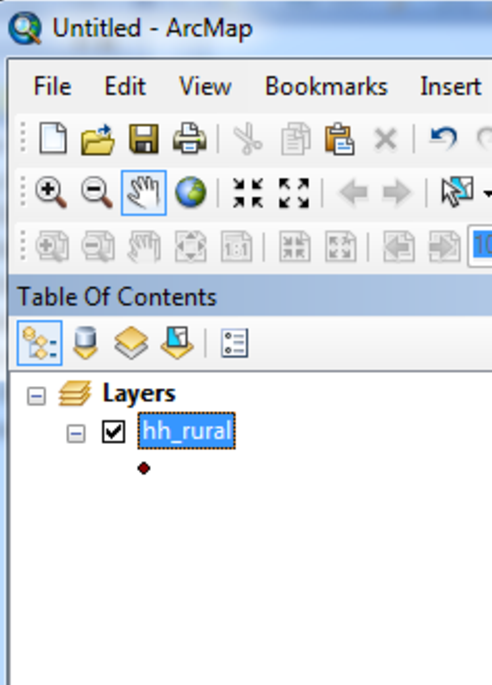
\includegraphics[scale=0.8]{figures/layerExample.pdf}
	\end{center}
\end{figure}

But those layers are just part of your .mxd Map Document -- when you delete the map document, they disappear, and by default they never exist as separate files on your hard drive like shapefiles or feature classes (you can save layers to a .lyr file, but most of us never do this). 

Personally, I like to think of a layer as being akin to a sticky note. When I’m writing a paper, I place sticky notes on books I’m using with information about chapters that might be useful to quote. Just as a layer is useless without its associated data file, the sticky note doesn’t actually have any value without its associated book. And when I finish the project I’m working on, the sticky is something I throw away, while the book I put back on my bookshelf -- just as layers disappear when a Map Document is deleted or not saved, even though your shapefiles and feature classes live on.



\subsection*{Layers in ArcPy}

What makes layers particularly complicated in ArcPy is that layers don’t usually exist as separate files on your harddrive. Rather, at least by default, any layers you create during your ArcPy session are automatically deleted as soon as your code finishes running. So for example, if you take a table of GPS coordinates and create an XY Layer of those coordinates, you need to then copy that layer into a Feature Class if you want to use the mapped GPS coordinates later.

But here's where things get a little complicated: layers that ``live'' in different places are handled differently by ArcPy. In particular, we can think of layers living in three places:
\begin{enumerate}
	\item \textbf{Native-ArcPy Layers:} If you create a layer in your ArcPy session, that layer lives in your ArcPy session, and will disappear as soon as your code stops running if you don't copy it into another format. 
	\item \textbf{.mxd Layers:} as noted in Section~\ref{cartography}, ArcPy has the ability to manipulate .mxd documents. As part of these manipulations, you can use ArcPy to \emph{reach into an .mxd document and modify the layers living in that .mxd document}.
	\item \textbf{.lyr Layers:} Finally, as noted above, it is possible to save a layer to your hard drive as a .lyr file. 
\end{enumerate}

In classic Arc fashion, in most documentation, these are all just called ``layers,'' but not all tools will work on all of these types of layers. In particular, the tools in the \emph{mapping} library (tools you run by typing arcpy.mapping.[functionName] instead of just arcpy.[functionName]) are only designed to work on .mxd Layers and .lyr Layers -- not native-ArcPy layers. But some tools (like ``SelectLayerByAttribute\_management()'') will operate on all three types of layers! I know, right?!

Basically, I can't give you guidance on all issues you may run into with Layers, \textbf{but so long as you recognize that when you see the term ``layer'' in help documentation, it may be referring to any one of these three types of layers -- native ArcPy layers, layers in .mxd files, or layers saved as .lyr files -- hopefully you can figure things out.}


\section{Selections}
As in ArcMap, ArcPy can also keep track of feature selections in layers (Yes, all three types of layers, but not shapefiles or feature classes!) To work with selections, we only really need three major tools: SelectLayerByAttribute\_management() and SelectLayerByLocation\_management(). SelectLayerByAttribute\_management() and SelectLayerByLocation\_management() allow manipulation of the selections of features in that layer. 

Note that SelectLayerByAttribute\_management() and SelectLayerByLocation\_management() are multifaceted tools -- the second argument allows you to specify whether you're creating a new selection, clearing an old selection, or modifying an existing selection, so it's really all we need. For syntax, just google these commands and check out the ESRI site!



\section{Other Style Points}\label{morestyle}
A couple more style points which are less important than those mentioned above, but which are still useful, particularly when you look at other people's code!

\subsection*{\textbf{Storing Filepaths as variables}}
Many ArcPy programmers don't like to ever use filepath strings as input to arguments; instead they store them in variables, then use the variables. The main value of this strategy is that if you're using the $myFeatureVariable$ a lot, and at some point you change the folder in which it is located, you only have to change the file location once. For example:

\begin{quote}
\begin{verbatim}
> WGS84 = arcpy.SpatialReference('WGS 1984')
> myFeatureVariable = "Z:/Documents/VAM/myDatabase.gdb/myExampleFeature"
> arcpy.DefineProjection_management(myFeatureVariable,WGS84)
\end{verbatim}
\end{quote}
Note that the myFeatureVariable is not enclosed in quotes!

\subsection*{\textbf{Named Arguments}}
This is optional, but it's another trick I really like for readability. By default, functions know how they're supposed to use each argument you pass them on the basis of the order they appear. For example, ``DefineProjection\_management(myFeatureVariable,WGS84)'' knows that myFeatureVariable is the target feature class because it is first, and WGS84 is the coordinate system to apply because it's second. But there is another way -- named arguments. 

In Section 3, we saw that the ESRI help page referred to each argument for an ArcPy function with a name. For DefineProjection, they're called $in\_dataset$ and $coor\_system$: 

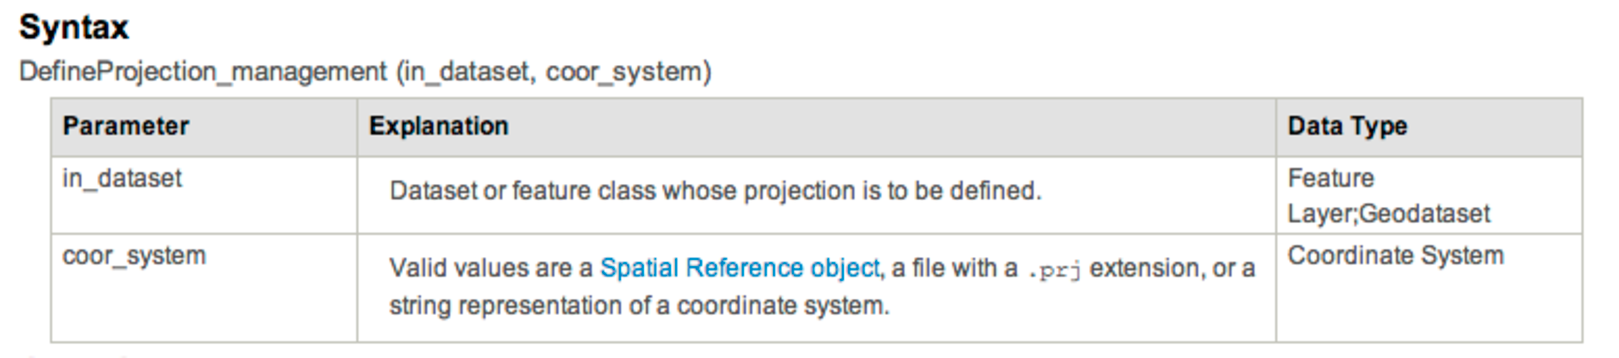
\includegraphics[scale=0.6]{figures/defineprojection.pdf}

Well, it turns out we can actual use those names to identify arguments. So instead of writing: 
\begin{quote}
\begin{verbatim}
> arcpy.DefineProjection_management(myFeatureVariable,WGS84)
\end{verbatim}
\end{quote}
I could write: 
\begin{quote}
\begin{verbatim}
> arcpy.DefineProjection_management(in_dataset = myFeatureVariable, 
coor_system = WGS84)
\end{verbatim}
\end{quote}
In fact, when you use named arguments, the order doesn't matter, so I could also write: 
\begin{quote}
\begin{verbatim}
> arcpy.DefineProjection_management(coor_system = WGS84, 
in_dataset = myFeatureVariable)
\end{verbatim}
\end{quote}

This provides two big advantages to the programmer. First, it makes code much more readable (since the names are informative). And second, some commands accept \emph{lots} of arguments, and if you only want to use the first, second, and 7th, you have to populate all the intervening spaces with $\#$s. For example, if you wanted to do a Spatial Join and use a custom search radius, you'd need to write:
\begin{quote}
\begin{verbatim}
> arcpy.SpatialJoin_analysis(USstates, Cities, StatesAndCities, "#",
 "#", "#","#", 1000)
\end{verbatim}
\end{quote}

But with named arguments, you'd be able to write:
\begin{quote}
\begin{verbatim}
> arcpy.SpatialJoin_analysis( target_features = USstates, 
join_features = Cities, out_feature_class = StatesAndCities, 
search_radius = 1000)
\end{verbatim}
\end{quote}

The first way is faster, but I prefer the second method given how much easier it is to understand when you go back to it. 

\section{Summary}
Good Style:
\begin{itemize}
	\item Start projects by copying source data to working directory
	\item Working directories
	\item Use SpatialReference
	\item Use variables for files
	\item Use named arguments
\end{itemize}

If you have problems, remember:
\begin{itemize}
	\item Check for schema locks
	\item Google the error -- ArcGIS errors are often mysterious
	\item There are \emph{three} things referred to as \emph{Layers}
\end{itemize}


\end{document}
